\chapter{Analýza}
V~první kapitole jsme specifikovali cíle naší práce, tedy implementaci platformy založené na herním enginu UrhoSharp umožňující tvorbu RTS her a~jejich distribuci. V~této kapitole popíšeme problémy při implementaci této platformy, námi zvolená řešení a~jejich alternativy.

\section{Herní engine}
Jak jsme napsali v~sekci \ref{sec:cileprace} Cíle práce, naším cílem je vytvořit platformu pro tvorbu RTS her za použití herního enginu UrhoSharp. \textit{\uv{UrhoSharp je multiplatformní 3D a~2D engine který může být použit pro tvorbu animovaných 3D a~2D scén za použití modelů, materiálů, světel a~kamer} } \citep{site:urhosharp}, jak říká úvodní stránka dokumentace enginu. Jak už název napovídá, UrhoSharp je .NET binding pro Urho3D engine \citep{site:urho3D}, což je opensource herní engine implementovaný v~C++.

Tento engine a~jeho binding do jazyka C\# jsme si vybrali především kvůli tvůrcům .NET bindingu, společnosti Xamarin, která je také autorem implementace .NET Frameworku Mono. V~rámci tohoto vztahu očekáváme největší podporu práce s~managed kódem, například jeho načítáním za běhu, na čemž je postaven náš systém pluginů. 

Jak uvidíme v~následující části, přestože je engine UrhoSharp navržen pro platformu Mono, nebylo na všech systémech možné překonat jejich omezení.

\section{Rozdíly systémů}
\label{sec:system_dif}
Hlavním cílovým systémem naší práce jsme se rozhodli zvolit systém Windows, především kvůli nejrozsáhlejší podpoře frameworku .NET, dále kvůli zřejmým výhodám ovládání pomocí klávesnice a~myši, a~v~neposlední řadě kvůli naší zkušenosti s~tímto systémem. Pro podporu dalších platforem je naším cílem vytvořit návrh platformy umožňující co nejjednodušší rozšíření na tyto systémy. Herní engine a~platforma .NET sice mnohé rozdíly systémů abstrahují a~umožňují multiplatformní řešení, existují ovšem oblasti, které i~při využití těchto abstrakcí vyžadují pro každý systém specifické řešení.  

Implementace pro mobilní systémy (iOS, Android) naráží oproti PC systémům na několik problémů, vycházejících především z~rozdílných operačních systémů, velikostí obrazovek a~způsobu přijímání vstupu od uživatele. Rozdíly mezi PC systémy (Windows, různé distribuce Linuxu, macOS) nejsou tak rozsáhlé, přesto se mohou vyskytnout problémy především kvůli různým implementacím frameworku .NET používaným mimo systém Windows.

Při řešení těchto problému jsme narazili na rozdíly, specifika a~omezení, které v~následujících částech přiblížíme.

\subsection{Zobrazení a~ovládání}
Na mobilních systémech je vztah mezi GUI, tedy grafickým uživatelským rozhraním, a~ovládáním mnohem bližší. Oproti PC systémům je zde nejčastěji jediným možným vstupem dotyková obrazovka. GUI musí tedy sloužit jak pro zobrazení informací hráči, tak pro získání převážné většiny vstupu od hráče. Dalším rozdílem je velikost obrazovky, která je obecně mnohem menší než u~jiných systémů. Ze statistik zařízení od společnosti Google \citep{site:materialdesign} můžeme vidět, že rozpětí velikostí obrazovek tzv.~\uv{smartphonů} používajících systém Android sahá od úhlopříčky 3,5~palce po 6,4~palce, kde nejčastější velikostí je rozpětí od 5~palců po 6~palců. Oproti tomu nejčastější velikosti obrazovek laptopů sahají od 11~palců po 17~palců a~více. 

I~přes to, že herní engine umožňuje tvorbu grafického rozhraní použitelného na všech systémech, různé druhy vstupu a~velikosti obrazovek nutí nás i~potencionální tvůrce her na naší platformě k~výrazně odlišnému návrhu rozhraní pro mobilní systémy. Engine Urho3D poskytuje separátní vývojové prostředí pro návrh scén a~uživatelského rozhraní, které je následně možné exportovat do XML souboru, který je poté možné načíst za běhu hry pro zobrazení specifikovaných scén a uživatelského rozhraní. Tento postup lze použít k~definici uživatelského rozhraní specifického pro cílový systém dané verze aplikace, tedy naší platformy. Oproti tomu by tvůrci balíčků byli nuceni distribuovat definice rozhraní pro všechny systémy, ze kterých by poté za běhu vybírali podle aktuálního systému, nebo by byli nuceni vytvářet a~distribuovat několik separátních balíčků, cílených vždy pro jediný systém. 

Ukázku těchto problémů a~jedno z~možných řešení můžeme vidět na příkladu ze hry Hearthstone \citep{site:hearthstone}, kde  \ref{fig:hearthstone_mobile} ukazuje mobilní verzi hry a \ref{fig:hearthstone_pc} ukazuje PC verzi hry. Přestože návrh této hry je ideální pro přenos na mobilní zařízení, což můžeme vidět například ve velice podobném designu vlastní herní plochy v~obou verzích, existují mezi PC a~mobilní verzí viditelné rozdíly. Jedním z~rozdílů je pozice kamery, která je v~mobilní verzi umístěna mnohem blíže herní ploše. Toto je jedno z~možných řešení problému menší velikosti obrazovek mobilních zařízení, díky kterému budou herní prvky na těchto obrazovkách zobrazeny ve větší velikosti za cenu zobrazení menší části herního světa. Další součástí řešení problému velikosti obrazovek je velikost fontu, která je v~mobilní verzi mnohem větší než u~PC verze. Zároveň s~touto změnou musí být také provedena odpovídající změna designu karet a~oblastí, kde se písmo a~číslice vyskytují. Řešení problému vstupu pomocí dotykové obrazovky můžeme vidět na obrázku \ref{fig:hearthstone_mobile}, který ukazuje dva různé stavy hry. První stav, který můžeme vidět na obrázku \ref{fig:hearthstone_mobile_closed}, je navržen pro zobrazení celkového stavu hry a~pozorování nepřátelských tahů. V~tomto stavu jsou hráčovy karty zmenšené a~schované v~pravém dolním rohu obrazovky, kde nezakrývají žádnou část herní plochy. Při kliknutí na karty následně rozhraní přechází do druhého stavu, který můžeme vidět na obrázku \ref{fig:hearthstone_mobile_open}. V~tomto stavu jsou karty hráče přemístěny do centrální pozice a~zvětšeny. Tímto přemístěním sice zakryjí velkou část herní plochy, ale v~danou chvíli jsou právě tyto karty cílem hráčovi pozornosti a~jimi zakrytá plocha je pro něj irelevantní. Tento systém vytahovaní, přemisťování a~zvětšování ovládacích prvků aplikace je obecným trendem v~mobilních zařízeních, umožňujícím větší velikost ovládacích prvků za cenu většího počtu interakcí uživatele se zařízením oproti počtu interakcí v~PC verzi aplikace pro dosažení stejného cíle. Toto můžeme vidět na obrázku \ref{fig:hearthstone_pc}, který ukazuje stejnou situaci v~PC verzi hry. Mezi \ref{fig:hearthstone_pc_closed} a \ref{fig:hearthstone_pc_open} nejsou karty nijak přesouvány či zvětšovány a~jsou viditelné neustále, hráč tedy může zahrát kartu bez předchozího kliknutí na schované karty, čím ušetří oproti mobilní verzi jednu interakci.
\begin{figure}[!tbp]
	\centering
	\subfloat[Bez interakce hráče.]{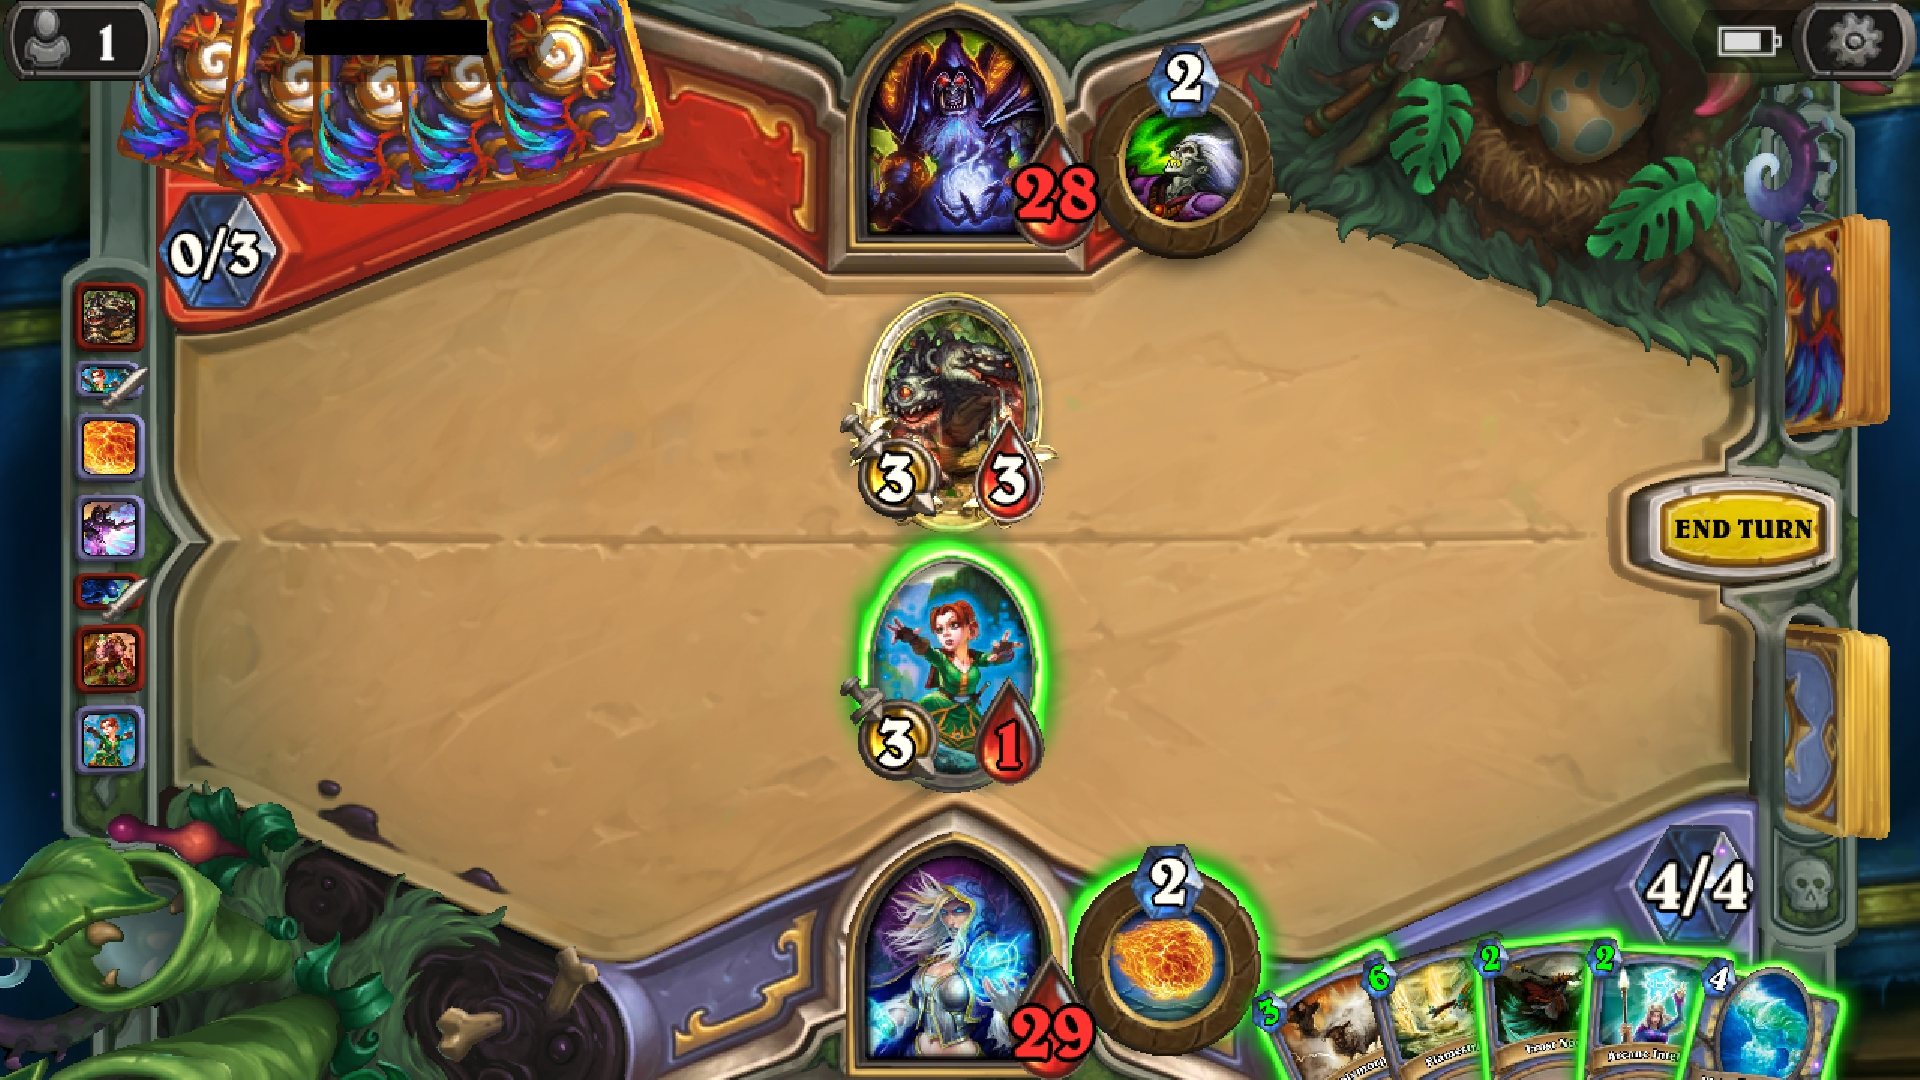
\includegraphics[width=0.47\textwidth]{hearthstone_mobile_closed}\label{fig:hearthstone_mobile_closed}}
	\hfill
	\subfloat[Při interakci hráče.]{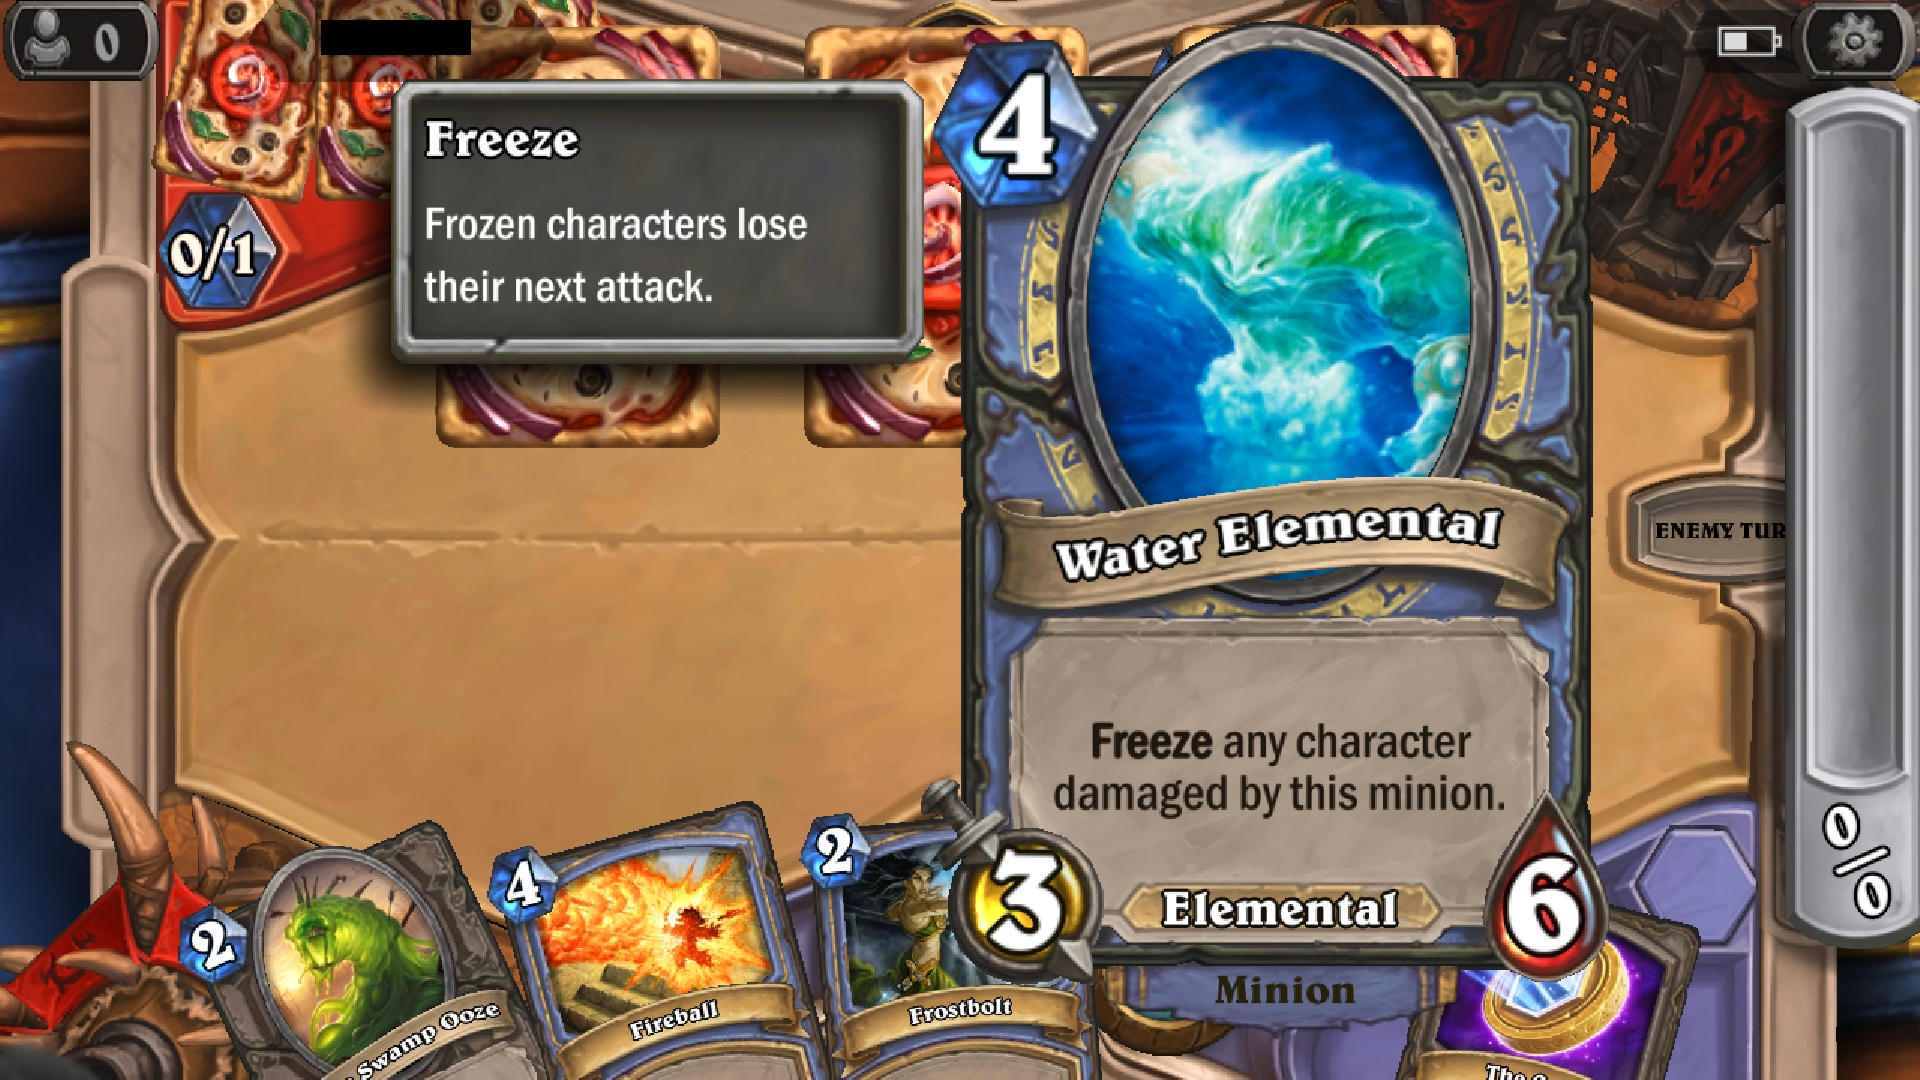
\includegraphics[width=0.47\textwidth]{hearthstone_mobile_open}\label{fig:hearthstone_mobile_open}}
	\caption{Uživatelské rozhraní mobilní verze hry Hearthstone.}
	\label{fig:hearthstone_mobile}
\end{figure}

\begin{figure}[!tbp]
	\centering
	\subfloat[Bez interakce hráče.]{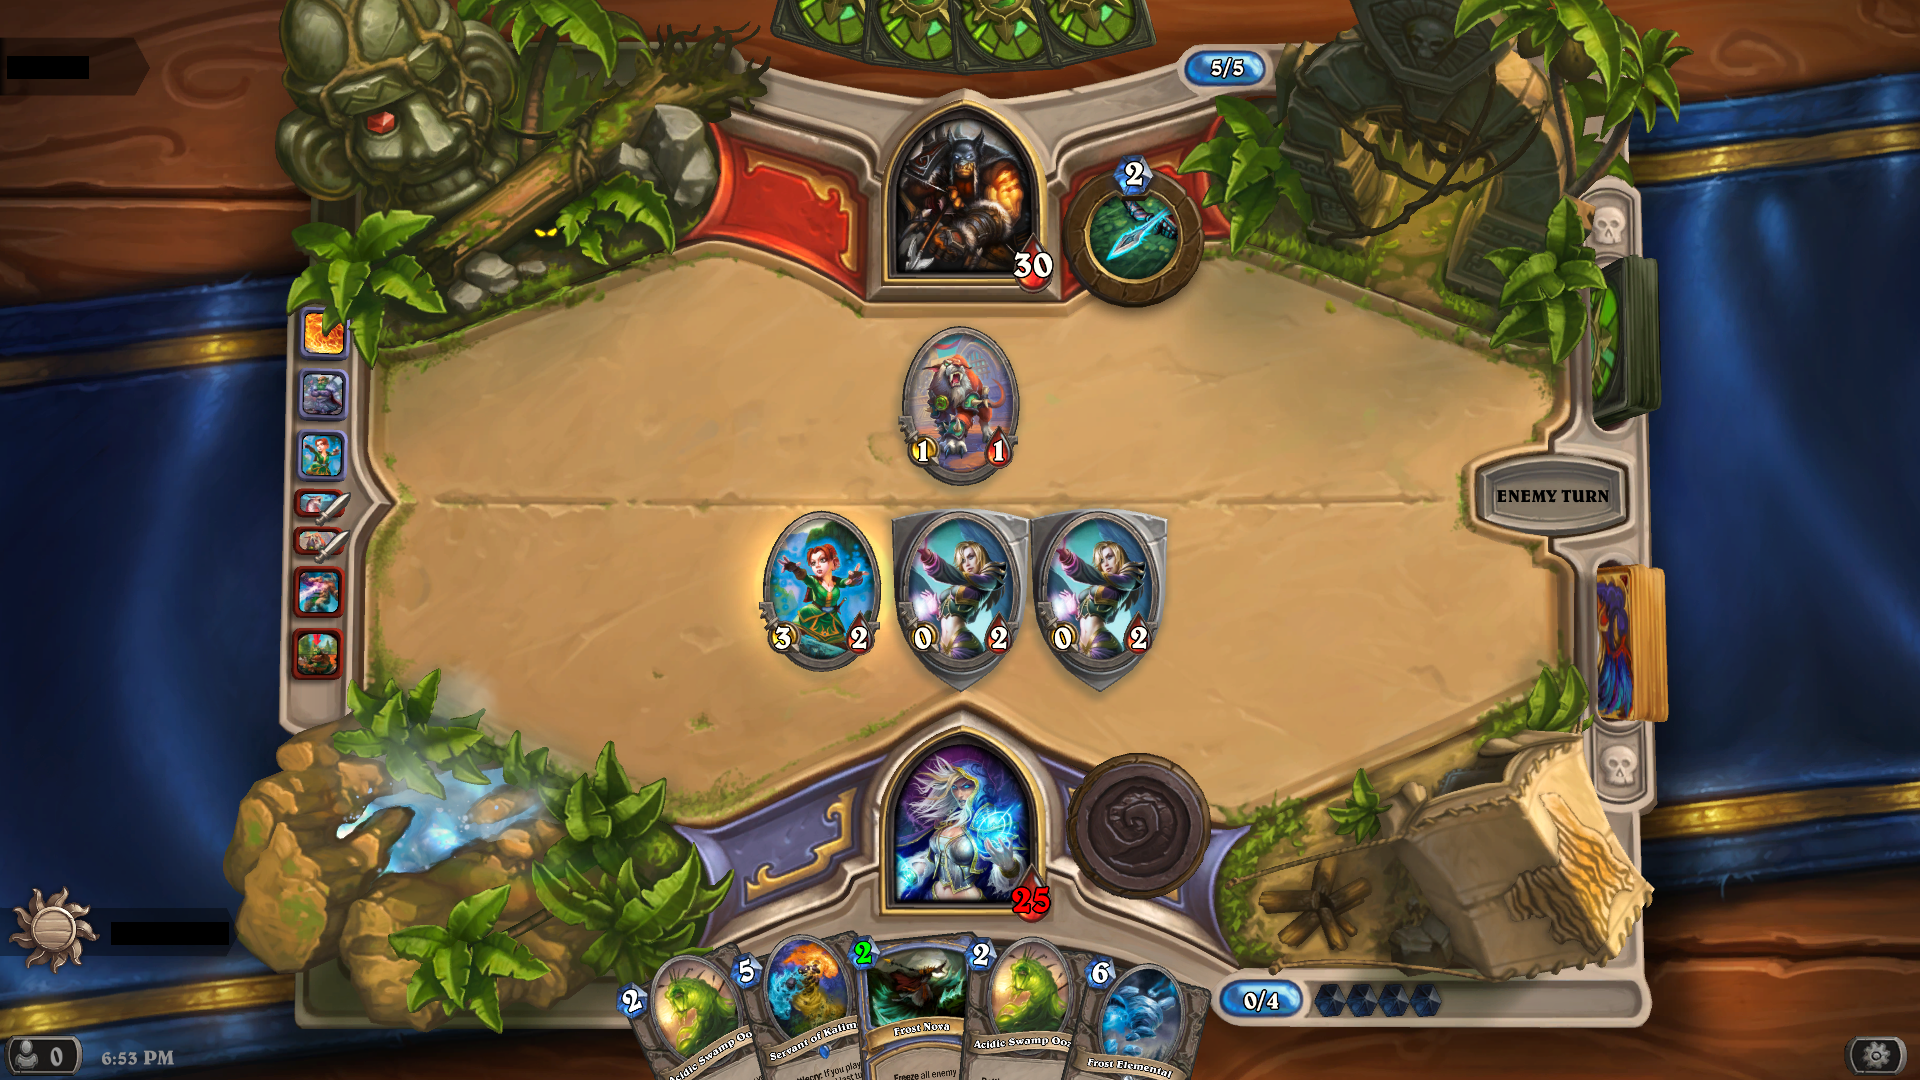
\includegraphics[width=0.47\textwidth]{hearthstone_PC_closed}\label{fig:hearthstone_pc_closed}}
	\hfill
	\subfloat[Při interakci hráče.]{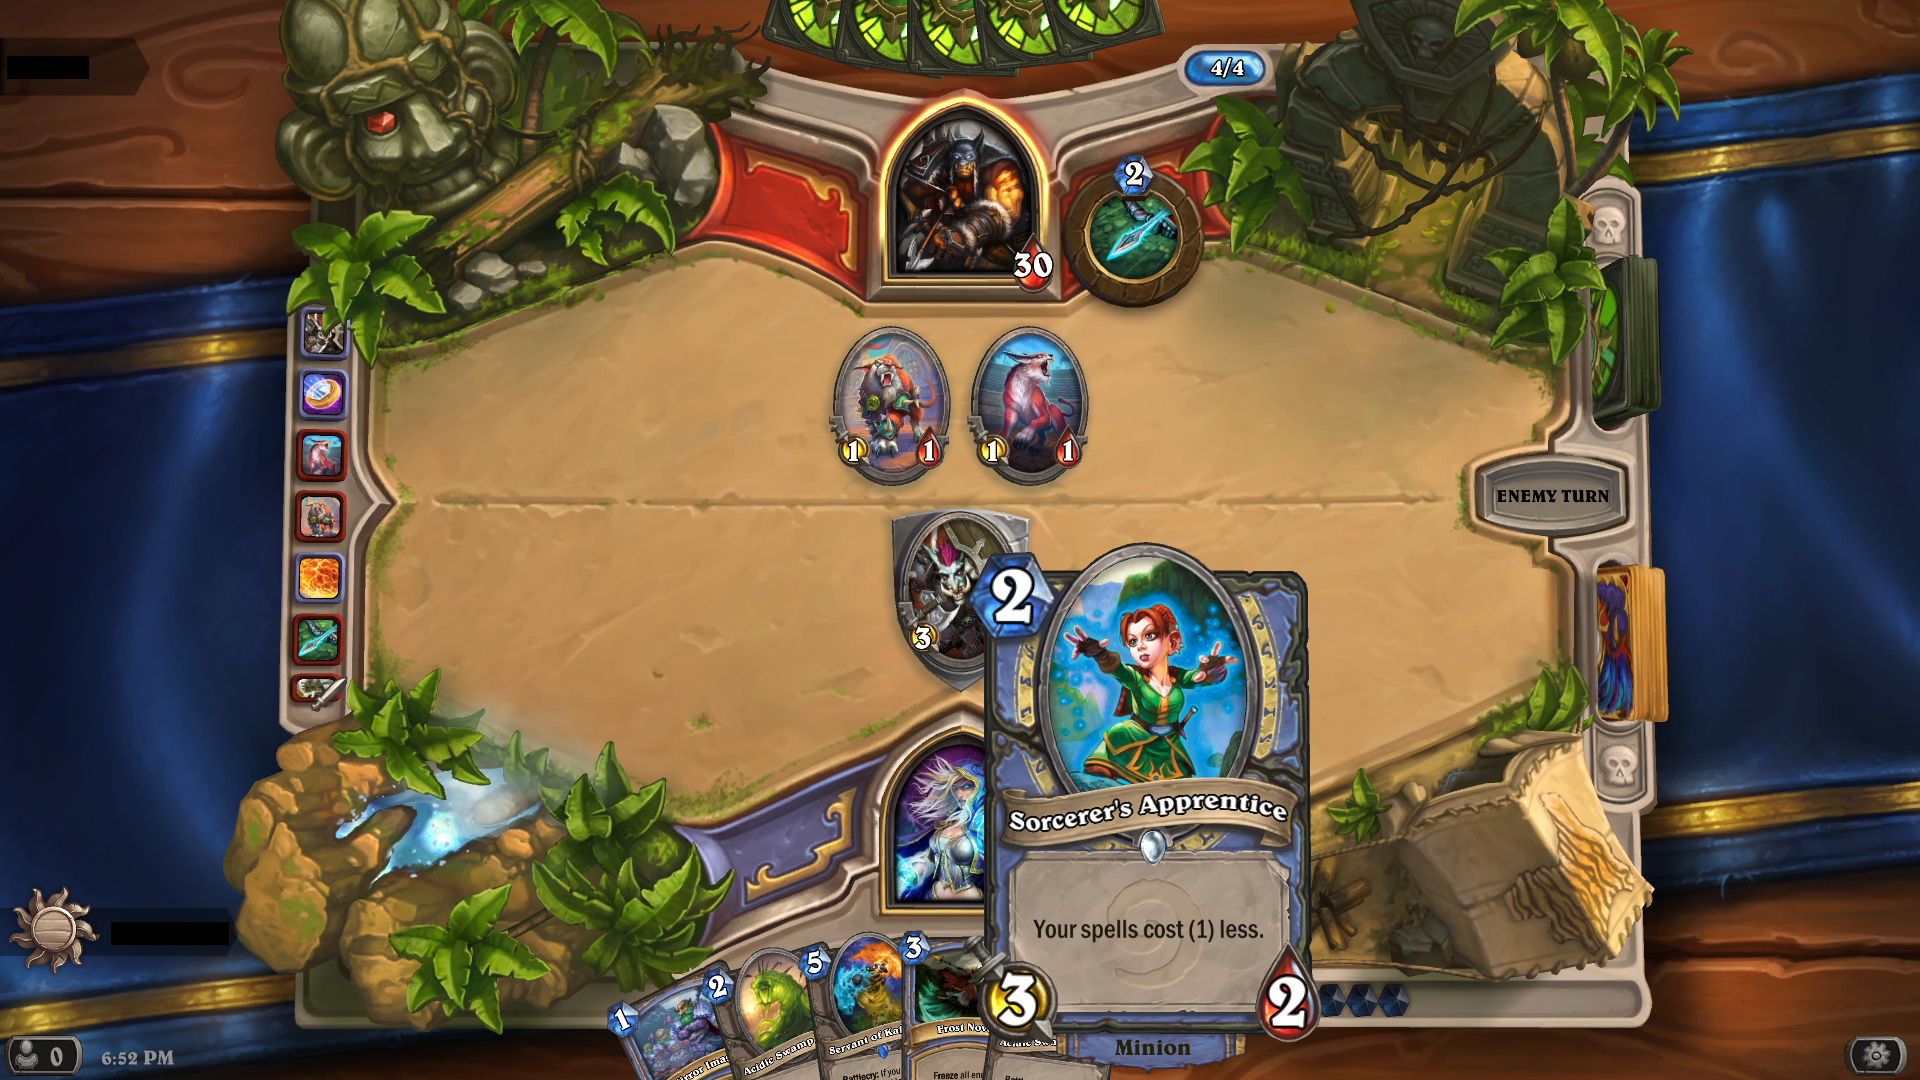
\includegraphics[width=0.47\textwidth]{hearthstone_PC_open}\label{fig:hearthstone_pc_open}}
	\caption{Uživatelské rozhraní PC verze hry Hearthstone.}
	\label{fig:hearthstone_pc}
\end{figure}

Jak můžeme vidět na příkladu ze hry Hearthstone \citep{site:hearthstone}, vedou nás problémy s~velikostí obrazovek a~dotykovým ovládáním k~separátnímu designu a~implementaci uživatelského rozhraní a~některých částí her. Pro tuto separátní implementaci jsme v~naší práci připravili základní kostru, upustili jsme ovšem od konečné implementace z~důvodu nedostatku času.

\subsection{Kompilace}
Dalším rozdílem, tentokrát s~rozdílným chováním i~mezi jednotlivými mobilními systémy, je jejich chování k~spustitelným souborům aplikací. Jak píší Joseph a~Ben Albahari \citep[str.~3,4]{book:cs7nutshell}, jsou jazyky cílené na platformu .NET překládány do \uv{Common Intermediate Language}  (CIL), z~kterého jsou obvykle až za běhu aplikace kompilovány do instrukční sady stroje, na kterém právě běží. Tento způsob se označuje jako \uv{Just-In-Time}  (JIT) kompilace, a~je standardním způsobem spouštění .NET aplikací. V~některých případech je ale použit jiný způsob, a~to tzv.~\uv{Ahead-of-time}  (AOT) kompilace, kdy je CIL kód ještě před distribucí zákazníkovy zkompilován do instrukční sady cílového stroje a~následně je distribuována tato již zkompilovaná verze. Tento způsob je používán pro zrychlení odezvy při větších velikostech assembly, čímž se předchází zpoždění v~důsledku kompilace CIL kódu. Další využití, zde již ne pouze za účelem optimalizace, ale vynucené systémem samotným, je při distribuci na systém \emph{iOS} \citep{site:aot}. Jak je napsáno v \textit{iOS Security Guide pro iOS verze 12.1} \citep[str.~27]{book:iossecurityguide}, není možné alokovat paměť zároveň jako \textit{\uv{writable} }, tedy s~možností do ní zapisovat, a \textit{\uv{executable}}, tedy s~možností v~ní uložená data vykonávat přímo jako instrukce procesoru. Tato skutečnost vylučuje jakékoli použití JIT kompilace, která používá právě takto namapované stránky jako výstup kompilace z \textit{intermediate} jazyka, tedy například CIL, do instrukční sady procesoru. Výjimkou jsou aplikace společnosti Apple, podepsané jejich klíčem, kterým je umožněna jedna alokace (jedno zavolání funkce \texttt{mmap}) takto namapovaných stránek. Tato výjimka je použita ve webovém prohlížeči Safari pro implementaci Javascript JIT kompilátoru.  

Tato skutečnost znemožňuje naší platformě jednoduché nahrání assembly pomocí reflexe a~nutila by nás k~složitějšímu řešení, které by se podle aktuálního systému muselo rozhodovat, kterou verzi assembly nahrát. Navíc by tento způsob nutil tvůrce balíčků přeložit svůj kód pro všechny možné architektury. Toto je důvod, proč jsme upustili od podpory systému iOS.

\subsection{Souborové systémy}
\label{sec:filesystems}
Každá aplikace má několik odlišných druhů souborů. Tyto druhy můžeme odvodit z~pro ně navržených adresářů ve Windows API \citep{site:knownfolders}, či z~implementace tohoto API v~platformě .NET \citep{site:specialfolders}. Těmito druhy souborů jsou:
\begin{itemize}
	\item \textit{Roaming user data} - data uživatele přítomná na všech počítačích v~síti, na které se může uživatel přihlásit;
	\item \textit{Local user data} - data uživatele lokální pro aktuální počítač;
	\item \textit{Private app data} - data aplikace přístupná pouze aplikaci;
	\item \textit{Public app data} - data aplikace přístupná všemi aplikacemi;
	\item \textit{Static app data} - neměnná data aplikace distribuovaná spolu s~aplikací.
\end{itemize} 

Některé z~těchto druhů souborů jsou na různých systémech sloučeny. Systém Android například nepodporuje více uživatelů, čímž ztrácí smysl rozdělovat uživatelská data a~data aplikace. Přístup aplikací k~souborovému systému je na tomto systému dále omezen. Jsou definována čtyři místa, kam může aplikace ukládat data \citep{site:androiddata}. Těmito místy jsou:

\begin{enumerate}
	\item \textit{internal file storage},
	\item \textit{external file storage},
	\item \textit{shared preferences},
	\item \textit{databases}.
\end{enumerate}

\textit{Internal file storage} je interní úložný prostor zařízení. Každá aplikace má zde systémem vytvořenou složku, do které má přístup pouze aplikace samotná. Tato složka je odstraněna při odinstalování aplikace.

\textit{External file storage} je \uv{externí}  úložný prostor, není tedy garantováno, že bude vždy přítomný. Tento prostor může být tvořen jak vestavěnou pamětí zařízení, tak fyzicky vyjímatelným prvkem, jako například SD kartou. Soubory na tomto úložišti jsou veřejně přístupné a~nejsou odstraňovány při odinstalování aplikace. 

\textit{Shared preferences} a \textit{Databases} slouží pro ukládání dat bez explicitního využití souborových systémů. Tento přístup k~datům nemá na PC systémech přímou podporu.


Dalším rozdílem mezi systémy je přístup k~souborům distribuovaným spolu s~aplikací, v~našem případě s~naší platformou. Na systému Android je každá aplikace distribuována jako \texttt{.apk} soubor. Formát Apk je zip archiv, obsahující všechny soubory naší aplikace, od kódu, přes assety, po preference. Tento archiv je v~duchu Linuxového VFS přímo namapován do stromu souborového systému viditelného z~naší aplikace. Bohužel .NET filesystem API nedokáže s~tímto mapováním pracovat, tedy není možné ho využít pro čtení těchto souborů. Řešením je využití Xamarin.Android zabalujícího Android Java API, které s~tímto archivem pracovat dokáže.

Přístup k~adresáři aplikace má další rozdíl, a~to v~zápisu do souborů. Na systému Android je zápis do těchto souborů úplně zakázán. Na PC systémech může být pro některé uživatele možné zapisovat do těchto souborů, ale aplikace by s~tímto přístupem neměla počítat.

Všechny tyto rozdíly při přístupu k~souborům nás nutí k~implementaci separátní komponenty pro práci se soubory, která je implementována pro každý systém zvlášť a~následně poskytována přenositelné části platformy.

\subsection{Shrnutí}
I~když je naším cílem pouze implementace pro systém Windows, ukázali jsme, že rozšíření na některé další systémy by nebyl problém a~nastínili jsme řešení možných problémů, které by při tomto rozšíření vznikly. Návrh naší implementace zohledňuje tato řešení a~umožňuje jejich  budoucí implementaci. Vzhledem k~velikosti implementace pro systém Windows nebudou ovšem tato řešení pro zbylé systémy součástí naší práce. Dále jsme zjistili, že systém iOS je neslučitelný s~požadavky naší aplikace a~rozšíření na tento systém tedy nebude možné.

\section{Formát a~načítání dat}
Důležitou součástí implementace naší platformy je systém balíčků pro distribuci vytvořených her. Tyto balíčky obsahují všechny součásti hry, od modelů a~textur, přes logiku a~umělou inteligenci, po mapy a~úrovně vytvořené tvůrcem hry. Všechny tyto součásti musí naše platforma být schopna načíst za běhu a~použít jak pro tvorbu nových map, tak pro hraní map již existujících.

\subsection{Struktura balíčku}
\label{sec:packagestructure}
Pro implementaci načítání balíčků musíme definovat strukturu, kterou budou balíčky splňovat, a~podle které bude platforma určovat typy souborů a~jejich závislosti.

První možností je založit strukturu balíčku na pevné adresářové struktuře, kde každý balíček bude tvořen jedním adresářem obsahujícím další pevně specifikovanou podadresářovou strukturu. Jednotlivé typy zdrojů, tedy 3D modely, textury, popis jednotek nebo skripty, by následně byly rozděleny a~identifikovány touto adresářovou strukturou. 

Pro popis typů jednotek, budov, projektilů, dlaždic a~nepřátel jsme se inspirovali v~existujících hrách, ať už Civilisation~V \citep{site:civ5} nebo Kerbal Space Program \citep{site:ksp}, a~využili jsme XML soubor pro definici vlastností a  závislostí. Dalšími možnostmi pro popis typů entit bylo využít formát JSON nebo dokonce definovat vlastní formát. Oproti ostatním zmíněným formátům má formát XML vestavěnou podporu přímo v~platformě .NET. Navíc tento formát umožňuje automatickou validaci vůči schématu, což nám ulehčí  validaci načtených dat. Možnou výhodou formátu JSON je jeho expresivita, umožňující minimalizovat velikost souborů. Vzhledem k~velikosti ostatních druhů dat jsme ovšem usoudili, že tato výhoda není dostačující pro volbu tohoto formátu. 

Implementace pomocí pevné adresářové struktury a~XML souborů pro popis typů entit ovšem vedla ke dvěma problémům. Prvním bylo velké množství malých XML souborů, jejichž správa by mohla vést k~častým omylům a~následným chybně pojmenovaným souborům, špatným cestám a~chybějícím souborům. Druhým problémem bylo přidávání balíčku do běžící hry. Hráč by mohl sice specifikovat adresář reprezentující balíček, následné ověření, zda je tento balíček korektní a~lze ho nahrát by nás ale nutilo k~procházení adresářové struktury, k~pokusům o~načtení souborů a~jejich validaci. Takováto implementace by byla pomalejší, náročnější na správu a~náchylnější k~chybám. 

Řešením bylo vytvořit centrální XML soubor, definující celý balíček. Všechny typy jednotek, budov, projektilů, nepřátel, logik úrovní, všechny úrovně obsažené v~balíčku a~další vlastnosti jsou popsány v~tomto souboru pomocí stejného XML, jakým byly popsány v~separátních souborech. Následně všechny assety, tedy modely, textury či assembly mohou být specifikovány relativní cestou vůči adresáři obsahujícímu tento jeden XML soubor. Tímto způsobem lze replikovat předchozí uspořádání, kde je každý typ assetů rozdělen do vlastního adresáře, ale navíc tento způsob umožňuje tvůrci balíčku specifikovat vlastní rozdělení a~umístění assetů. Zároveň toto uspořádání ulehčuje přidání balíčku a~ověření jeho korektnosti, kde stačí, aby uživatel zadal cestu k~tomuto XML souboru, a~pouhou validací podle schématu lze ověřit jeho validitu.

Naším finálním řešením je tedy reprezentovat každý balíček jedním XML souborem, který dále obsahuje relativní cesty odkazující na zbylý obsah balíčku. Tento soubor má formát daný pevným schématem a~tento formát je kontrolován při každém načtení tohoto souboru. 

\subsection{Data entit}
Nyní již víme, jak data rozdělit a~odkazovat na ně. Nyní musíme určit, jaká data budeme u~jednotlivých typů entit požadovat a~jaká vlastní data umožníme tvůrcům her si zde uložit. Naším cílem je umožnit specifikování typů entit a~k~nim náležejících dat, definujících vlastnosti těchto typů entit. 

Naše platforma bude poskytovat funkcionalitu společnou většině her typu specifikovaného v~úvodní části \ref{sec:uvod}. 
Tato funkcionalita zahrnuje:
\begin{enumerate}
	\item načítání pluginů a~volání jejich metod,
	\item uživatelské rozhraní,
	\item správa balíčků,
	\item vykreslování herního světa.
\end{enumerate} 

Naše platforma bude vynucovat specifikaci nezbytných dat pro implementaci poskytované funkcionality. Těmito daty jsou:
\begin{enumerate}
	\item assembly;
	\item ikony, barvy pro zobrazení na minimapě;
	\item identifikátory a~jména balíčků, typů entit, úrovní, logik hráčů;
	\item 3D modely, textury, animace.
\end{enumerate}
Protože jsou tyto vlastnosti společné většině entit v~námi podporovaných typech her, nahrává naše platforma automaticky zde specifikované vlastnosti při vytvoření entity v~herním světě a~následně je využívá pro implementaci poskytovaných vlastností.

Dále umožníme přidat libovolná další data do XML elementu reprezentujícího typ entity pro použití tvůrcem hry v~jeho implementaci logiky. Tato data nebude naše platforma nijak validovat, pouze je při vytvoření entity v~herním světě předá načítanému pluginu implementujícímu logiku vytvářené entity. Bude pouze na tvůrci této logiky, aby získaná data validoval a~následně z~nich inicializoval logiku či použil systém výjimek k~oznámení chyby v~datech. Tento způsob implementace umožní tvůrcům vytvářet universálnější logiku, jejíž chování budou schopni modifikovat právě načítanými daty ze souboru. Bez této funkcionality by byli tvůrci her nuceni všechna data přesunou z~XML souboru přímo do kódu logiky.

\subsection{Formáty assetů}
V~předešlé části jsme popsali, jak náš systém balíčků umožňuje zaznamenat umístění dat potřebných pro spuštění úrovně. V~této části dále upřesníme, jakých formátů můžou tato data být a~jaká jsou omezení při použití určitých formátů dat. Slovem \textit{\uv{asset} } označujeme jakákoli data, která může tvůrce hry poskytnout naší platformě a~použít je při tvorbě hry. Tato data lze rozdělit do několika kategorií:
\begin{itemize}
	\item grafická data,
	\item logika a~pluginy,
	\item ostatní.
\end{itemize}

V~následujících částech popíšeme jednotlivé kategorie dat, jejich formáty a~využití.

\subsubsection{Grafická data}
Mezi grafická data patří především 3D modely a~k~nim náležící textury a~animace. Podporované formáty těchto dat jsou omezeny námi používaným herním enginem UrhoSharp (Urho3D). Tento engine interně používá knihovnu Open Asset Import Library (Assimp) \citep{site:assimp}, která umožňuje načítání mnoha formátů 3D modelů do uniformní reprezentace, která je následně používána enginem samotným.

Dalšími grafickými daty používanými naší platformou jsou textury dlaždic. Každý typ dlaždic, jak je popsáno v~části \ref{sec:packagestructure} o~struktuře balíčku, je definován XML elementem v XML souboru balíčku. Tento element povinně specifikuje texturu, představující vzhled dlaždic tohoto typu. Kvůli naší implementaci zobrazení mapy, blíže popsaného v~části \ref{sec:mapimpl}, musí být tato textura manipulovatelná z~C\# kódu naší platformy. Bohužel engine Urhosharp v~aktuální verzi neposkytuje přístup k~dekompresi textur, implementované enginem Urho3D. Z~tohoto důvodu není možné využít komprimované formáty textur pro vzhled dlaždic.

Dalšími povinnými grafickými daty, které naše platforma požaduje, jsou textury ikon pro jednotky a~budovy. Pro každý z~těchto dvou druhů entit požadujeme texturu, která je následně použita při implementaci nástrojů  poskytovaných naší platformou, umožňujících editaci a~hraní úrovní. Tyto nástroje umožňují umisťovat jednotky a~budovy do editované úrovně a~dále při jejím hraní vybírat skupiny jednotek a~vydávat jim rozkazy. Definice každého typu jednotky nebo budovy následně obsahuje specifikaci části těchto textur, která má být využita pro reprezentaci tohoto konkrétního typu. Přestože platforma umožňuje tvůrcům her implementovat vlastní nástroje pro editaci a~hraní her, předpokládáme, že i~tyto nástroje budou mít potřebu reprezentovat jednotlivé druhy jednotek a~budov a~využijí k~tomu právě tyto ikony.

Grafická data obsažená v~balíčku nejsou omezena pouze na platformou požadovaná a~používaná data, ale je umožněno tvůrci přibalit libovolná data podporovaná enginem UrhoSharp a~následně je využít při tvorbě hry. Díky tomu, že mají tvůrci her plný přístup k~schopnostem enginu UrhoSharp, mohou, stejně jako platforma, za běhu použít tato data pro úpravu vzhledu jednotek, budov či projektilů, případně pro rozšíření grafického uživatelského rozhraní. Mezi tato data patří například \textit{Shadery} a~animace.

\subsubsection{Logika a~pluginy}
\label{sec:logicandplugins}
Jak jsme uvedli v~části \ref{sec:requirements}, jedním z~hlavních cílů naší práce bylo umožnit využití jazyka C\# pro skriptování logiky hry a~umělé inteligence nepřátel. Díky využití herního enginu UrhoSharp, postaveného nad frameworkem .NET, máme zajištěno, že v~naší implementaci budeme schopni použít systém \textit{Reflection} pro načítání a~používání pluginů. 

I~v~případě, že by naše práce nevyužívala engine UrhoSharp či jiný engine postavený na platformě .NET, bylo by možné použít jazyk C\# pro skriptování. Taková implementace, využívající jiný jazyk pro tvorbu platformy, by byla nucena využít jazyk C++/CLI pro vytvoření \uv{mostu}  mezi kódem tvořícím platformu a~managed kódem, umožňujícím nahrávání pluginů za běhu a~jejich využití z~kódu platformy. Tato alternativa je ovšem mnohem složitější na implementaci než je tomu při použití enginu založeného na frameworku .NET. Při použití herního enginu připraveného pro .NET, jako je právě UrhoSharp, je možné tvůrcům pluginů navíc poskytnout plnou sílu tohoto enginu a~umožnit jim využít všechny jeho schopnosti bez jakéhokoli zásahu či manuálního zprostředkovávání. V~případě využití enginu v~jiném jazyce by musel \uv{most}  explicitně implementovat všechny schopnosti enginu, které by chtěl poskytnout tvůrcům pluginů a~přeposílat každý požadavek vlastnímu hernímu enginu.

Obě předešlá řešení využívají systém \uv{Reflection}  pro načítání tvůrcem dodaných assembly, nalezení tříd odpovídajících jednotlivým jednotkám, vytvoření instancí těchto tříd a~jejich následné použití. Pojmem \uv{Reflection}  označujeme sadu tříd .NET frameworku umožňujících introspekci .NET assembly, poskytující informace o~třídách obsažených v~těchto assemblies, jako například implementovaná rozhraní, poskytované metody či obsažené atributy. \uv{Reflection}  dále umožňuje načítání existujících assembly za běhu programu, či dokonce generování nových assembly. 

Assembly jsou identifikovány jménem, verzí, \textit{culture} a~veřejným klíčem. 
Při načítání je assembly nahrána do tzv.~kontextu. Existují čtyři kontexty, do kterých jsou assembly nahrávány. Těmito kontexty podle popisu v dokumentaci .NET frameworku jsou \citep{site:assemblyload}:
\begin{itemize}
	\item \textit{Default Load Context}
	\item \textit{Load-From Context}
	\item \textit{Reflection-only Context}
	\item \textit{No Context}
\end{itemize}

\textbf{Reflection-only} context slouží pouze pro zkoumání metadat assembly pomocí reflection a~znemožňuje vykonání kódu do tohoto kontextu nahrané assembly, proto je pro nás nezajímavý a~dále ho nebudeme rozebírat.

\textbf{Default Load Context} je kontext, ve kterém je nahrána assembly naší aplikace a~všechny její závislosti. Do tohoto kontextu lze manuálně nahrávat další assembly, pokud se tyto assembly nachází v \textit{Global assembly cache} (\emph{GAC}), v~adresáři aplikace (\textit{applicationBase}) nebo v~aplikací specifikovaných podadresářích \textit{applicationBase} (\textit{PrivateBinPath}). Pokud je identická assembly již nahrána, nenahrává se znovu ale vrací se reference na již nahranou assembly. Závislosti nahrávaných assembly jsou automaticky vyhledávány na těchto třech místech.

\textbf{Load-From Context} je kontext, do kterého jsou assembly nahrávány pomocí metody \texttt{Assembly.LoadFrom}. Do tohoto kontextu lze nahrát assembly specifikováním cesty spolu s~výše zmíněnými vlastnostmi identifikujícími assembly, a~tato cesta je přidána jako pátá identifikační vlastnost. Tímto způsobem lze nahrávat assembly ležící mimo \emph{GAC}, \textit{applicationBase} a \textit{PrivateBinPath}. Závislosti jsou hledány nejdříve mezi již nahranými assembly v \textit{Default Load Contextu}, následně v~adresáři, ze kterého byla assembly nahrána a~nakonec na cestách pro nahrávání assembly do \textit{Default Load Contextu}.

\textbf{No Context} je využíván při načítání  assemblies vygenerovaných pomocí \texttt{Reflection.Emit} a \texttt{Assembly.LoadFile}. Navíc je toto jediný způsob, jak načíst dvě verze té samé assembly. Pod pokličkou je vytvořen každé nahrané assembly zvláštní privátní kontext. Problémem tohoto kontextu je, že nejsou automaticky nahrávány závislosti. Tedy nezbývá nic jiného než závislosti nahrát manuálně, buď před načtením assembly nebo odchycením \texttt{AssemblyResolve} události.

V~naší platformě používáme \texttt{Assembly.LoadFrom}. Tento způsob nám umožňuje nahrávat assembly z~libovolných podadresářů uvnitř tvůrci tvořených balíčků, bez omezení na jejich adresářovou strukturu. Díky načítání závislostí ze zdrojového adresáře assembly mohou tvůrci her přibalit jimi používané knihovny do balíčku, které budou následně při použití automaticky načteny.

Alternativou použití \texttt{Assembly.LoadFrom} by bylo nutit tvůrce balíčků specifikovat cesty, ve kterých se mohou vyskytovat assembly, a~tyto cesty následně přidat do \textit{PrivateBinPath}. Tento přístup by ovšem omezil místa, ve kterých může naše platforma mít umístěné balíčky, na podstrom adresáře, ve kterém je umístěna naše platforma. Jak jsme psali v~části \ref{sec:filesystems} o~rozdílech souborových systémů, některé ze systémů nepodporují změny v~adresářového podstromu aplikace a~není tedy možné do tohoto podstromu umístit balíčky. I~na systémech, na kterých je možné zapisovat do podstromu aplikace, není tento přístup k~souborům považován za dobrý design, jak říká tento, i~když poněkud zastaralý, návod pro umisťování souborů na systému Windows \citep{site:windowsappfiles}. Hlavním důvodem je omezení přístupových práv, které systém uvaluje na standardní cíl instalace aplikací.

Naše aktuální implementace nijak neřeší uvolňování assemblies ve chvíli, kdy hra končí a~hráč načítá jiný balíček. Vzhledem k~velikosti assembly v~paměti by ale toto neměl být při běžných počtech používaných balíčků problém. Vzhledem k~budoucí unifikaci .NET Frameworku, .NET Core a~Mono pod implementací .NET 5 \citep{site:dotnet5}, který je následníkem .NET Core, není v~této chvíli jednoduché zvolit způsob uvolňování nepoužívaných assembly. Aktuální způsob v~námi používaném .NET Framework je použití \texttt{AppDomain}, pomocí které by bylo možné oddělit balíčky od sebe a~umožnit jejich uvolňování. Toto řešení ovšem není podporované v .NET Core, který funkcionalitu uvolňování assembly ze systému \texttt{AppDomain}, který není v~této verzi Frameworku podporován, přemisťuje do třídy \texttt{AssemblyLoadContext} \citep{site:assloadcontext}. Protože .NET 5 vychází z .NET Core, předpokládáme, že by v~budoucnu bylo možné využít právě \texttt{AssemblyLoadContext} pro řešení tohoto problému. 

\subsection{Formát uložených úrovní}
\label{sec:savingformat}
Ukládáním úrovně rozumíme serializaci aktuálního stavu hry a~uložení takto serializovaných dat do souboru. Pro serializaci jsme měli několik požadavků: 
\begin{enumerate}
	\item otevřenost schématu serializovaných dat,
	\item minimalizace velikosti serializovaných dat,
	\item rychlost serializace a~deserializace.
\end{enumerate}

Účelem prvního požadavku je umožnit tvorbu nezávislých editorů úrovní, importujících a~exportujících náš formát dat. Tento požadavek splňují serializace do formátu XML, definovaného pomocí \textit{XSD} schématu, a~binární serializace popsaná pomocí \textit{interface description language (IDL)}. Příkladem takovéto binární serializace je formát Protocol buffers \citep{site:protobuf} od společnosti Google. Z~binárních serializačních frameworků je pro jazyk C\# nejlépe podporován právě formát Protocol buffers, ať už použit sám o~sobě či za podpory knihovny protobuf-net, umožňující automatickou generaci IDL souborů z~anotací ve zdrojovém kódu. 

Druhý a~třetí požadavek nás vedl k~volbě binární serializace, která minimalizuje velikost dat a~má nejrychlejší zpracování. Tuto skutečnost sděluje jak dokumentace Protocol buffers \citep{site:protobufdevguide}, tak ji můžeme vidět experimentálně podloženou v~benchmarku Maxima Novaka \citep{site:serializationspeed}. Tímto jsme vybrali formát Protocol buffers, který lze v~jazyce C\# použít buď manuální specifikací \textit{\uv{message} } pomocí IDL, vygenerováním zdrojového kódu tříd v~jazyce C\# z~této specifikace a~následnou manuální serializací, nebo využitím knihovny Protobuf-net, která z~anotací ve zdrojovém kódu generuje specifikaci \textit{\uv{message} } a  metody pro serializaci a~deserializaci dat.

Naším cílem bylo využití knihovny Protobuf-net, bohužel tato knihovna vyžaduje v~případě použití dědičnosti, aby \textit{base} typy, tedy typy, od kterých se dědí, byly označeny atributem \texttt{ProtoInclude} \citep{site:protobufnet}. Vzhledem k~tomu, že všechny naše třídy reprezentující jednotky, budovy, projektily a~hráče, dědí od UrhoSharp třídy \texttt{Component}, není možné tyto třídy serializovat pomocí Protobuf-net. Tento problém lze řešit dvěma způsoby: 

\begin{enumerate}
	\item Separovat reprezentaci entit do dvou tříd. První třída, která bude potomkem třídy \texttt{Component} a~bude reprezentovat entitu v~grafu herní scény, a~druhá, která bude reprezentovat entitu z~pohledu logiky, s~kterou by pracovala naše platforma i~implementace pluginů, a~která by vlastnila a~ovládala první třídu. V~této reprezentaci by bylo možné využít Protobuf-net, znamenalo by to ovšem složitou delegaci volání mezi třídami a~možné problémy při využití grafu scény pro nalezení entity. 
	\item Využít pro serializaci přímo technologii protocol buffers, která je na pozadí používána knihovnou Protobuf-net, a~manuálně implementovat serializaci hry. Tato možnost se nám zdála jako lepší, protože nám také umožňovala manuálně specifikovat \texttt{.proto} soubory, z~kterých protocol buffers generují třídy umožňující serializaci a~deserializaci v~různých jazycích. Navíc nám tento postup umožňuje specifikovat přesnou posloupnost akcí při deserializaci.
\end{enumerate}

\section{Poskytovaná funkcionalita}
V~úvodní kapitole jsme vymezili druh her, které bude naše platforma podporovat, pomocí společných rysů a~funkcionality. Cílem naší platformy je poskytovat implementaci této společné funkcionality a~tím zjednodušit tvorbu her. Tato kapitola rozebere naši implementaci společné funkcionality, její výhody a~omezení, a~popíše možnosti modifikace chování těchto implementací z~uživatelského kódu.

\subsection{Mapa}
\label{sec:mapimpl}
Jednou z~hlavních funkcionalit poskytovaných naší platformou tvůrcům her je implementace herní mapy. Tato implementace poskytuje rozhraní pro dotazování na aktuální stav, manipulaci s~mapou a~grafickou reprezentaci zobrazenou hráči. Naše implementace odděluje logickou reprezentaci, která je poskytována zbylému kódu platformy a~kódu uživatelských pluginů, a~grafickou reprezentaci, která je vytvářena z~logické reprezentace a~zobrazována hráči. Toto rozdělení je určeno pro možné změny grafické reprezentace bez ovlivnění logické reprezentace a~na ní závislého kódu. 

\subsubsection{Logické rozdělení}
\label{sec:maplogic}
Mapa je ve hrách využívána pro zjišťování typu a~výšky terénu či přítomnosti entit, jako například budov a~jednotek, nejčastěji za účelem vyhledání cesty mezi dvěma pozicemi v~herním světě. Dalším možným důvodem pro zjišťování mapou poskytovaných informací může být zjištění viditelnosti mezi dvěma entitami, možnosti střelby mezi dvěma entitami či interakce hráče se skupinami entit.  Existuje několik způsobů, jak implementovat tyto funkce herní mapy.

V~úvodní kapitole jsme specifikovaly, jaké hry bude naše platforma podporovat. Z~vlastností těchto her nám vyplynula obdélníková mapa, rozdělená na čtvercové dlaždice. Toto ovšem není jediná možná implementace. V~této části popíšeme další možné typy implementací map, jejich výhody, nevýhody a~použití.

\textbf{Mapa bez rozdělení} vede při každém dotazu na přítomnost budov či jednotek v~dané oblasti mapy k~výpočtu průsečíků ploch zabíraných všemi jednotkami a~budovami s~danou oblastí mapy. Asymptotická složitost této operace je tedy O(N), kde N je počet budov či jednotek v~naší hře.

\textbf{Mapa s~rozdělením} na části umožňuje při dotazu na přítomnost jednotek či budov v~oblasti mapy prozkoumat pouze části tvořící tuto oblast mapy. Části, označovány jako \textit{\uv{Tiles} }, v~překladu dlaždice, mohou být různých tvarů. Nejčastějšími tvary jsou čtverec či šestiúhelník. 

Při rozdělení na čtverce lze mapu jednoduše uložit do dvourozměrného pole, což dále usnadňuje dotazy na prohledání oblasti mapy. Nevýhodou čtvercového tvaru dlaždic je různá vzdálenost sousedních dlaždic, pokud umožníme pohyb mezi všemi osmi sousedními dlaždicemi. Kde vzdálenost středů dlaždic sousedících celou hranou je rovna délce hrany, vzdálenost středů dlaždic sousedících pouze rohem je rovna \(\sqrt{2a^2}\), kde \textit{a} je délka hrany čtverce. Oproti tomu při použití šestiúhelníkových dlaždic je vzdálenost mezi všemi sousedy rovna. 

\subsubsection{Grafická reprezentace} 
\label{sec:mapgraphicsanalaysis}
Jak jsme popsali v~předešlé části, mapa je obdélníkového tvaru, rozdělena na čtvercové dlaždice o~velikosti 1x1. Existují dva základní druhy možných implementací grafického zobrazení takovéto mapy.

První možností, ilustrovanou obrázkem \ref{fig:mapbigtexture}, je vytvoření textury, ve které bude každé dlaždici odpovídat separátní část textury. Tuto implementaci nazýváme \uv{Textura dlaždic}. Velikost textury je závislá jak na velikosti mapy, v~obrázku značené \textit{m}, \textit{n} a~udávané v~počtu dlaždic v~daném rozměru, tak na velikosti textury jednotlivých typů dlaždic, zde značené \textit{k}. S~ohledem na čtvercový tvar dlaždic požadujeme i~po texturách jednotlivých typů dlaždic čtvercový tvar. Velikost výsledné textury bude rovna \(k^2 * m * n\). Tuto texturu můžeme vidět v~dolní části obrázku \ref{fig:mapbigtexture}. Na objekt reprezentující terén je následně tato textura promítnuta pomocí standardního \textit{UV} mapování, což je na ukázce reprezentováno šipkami mapujícími vrcholy geometrie na texturu. V~takovéto textuře má každá dlaždice přiřazenu disjunktní část textury, lze tedy vzhled jednotlivých dlaždic upravovat nezávisle na vzhledu ostatních dlaždic. Tímto způsobem lze vytvořit různé přechody mezi typy dlaždic a~provést další úpravy na celkovém vzhledu herní mapy. Ukázku takovýchto přechodů můžeme vidět na dlaždicích 1 a~2.
 
Nevýhodou této implementace je především velikost textury, která v~závislosti na velikostech textur jednotlivých typů dlaždic může dosáhnout stovek MiB až jednotek GiB. Takováto velikost textury by byla neúnosná i~pro slabší počítače, nemluvě o~mobilních zařízeních. Další nevýhodou této implementace je složitost změny typu dlaždice. Při změně typu je v~této reprezentaci nutné najít část textury odpovídající měněné dlaždici a~do této části nakopírovat texturu nového typu. Vzhledem k~velikosti textur dlaždic by tato operace mohla být časově velice náročná, především při změně typu velkého počtu dlaždic. Možnou výhodou této implementace je schopnost reprezentovat každý z~vrcholů, ve kterém se vyskytují rohy sousedících dlaždic, pomocí jednoho \uv{vertexu}, tedy grafického vrcholu. Díky tomu je omezena velikost \textit{vertex bufferů} a~zaručena spojitost mapy. Vzhledem k~velikosti textury je ovšem úspora paměti nedostatečná.

\begin{figure}[h]
	\centering
	\input{img/BigTextureMap.pdf_tex}
	\caption{Implementace pomocí textury dlaždic.}
	\label{fig:mapbigtexture}
\end{figure}

Druhou možností, ilustrovanou obrázkem \ref{fig:mapsmalltexture}, je vytvořit texturu, ve které bude textura každého typu dlaždic právě jednou. Tuto texturu, obsahující vzhled typů dlaždic, můžeme vidět v~levé dolní části obrázku. Velikost takovéto textury závisí oproti předchozí implementaci pouze na počtu typů dlaždic. I~když typů dlaždic může být neomezeně, nepředpokládáme, že by tento počet přesáhl malé stovky. Díky tomu je tato implementace paměťově mnohem úspornější. Při takovéto implementaci je poté každá dlaždice určitého typu namapována na stejnou část textury, což je na obrázku ukázáno na příkladu dlaždic 1 a~2. Vzhledem k~tomuto mapování všech dlaždic stejného typu na stejnou část textury nelze jednoduše vytvořit přechody mezi typy dlaždic, jak tomu bylo v~první implementaci. Jedinou možností je vytvořit separátní typ, který bude reprezentovat přechod mezi dvěma typy dlaždic. Další možnou nevýhodou této implementace je nutnost reprezentovat každou dlaždici separátní čtveřicí tzv.~\uv{vertexů}, tedy grafických vrcholů. Oproti první implementaci tedy bude pro reprezentaci mapy stejné velikosti potřeba čtyřnásobný počet vrcholů. Tato možná nevýhoda je ale vyvážena úsporou paměti v~rámci textury typů, dále díky jednoduší implementaci změny typů dlaždic, a~v~neposlední řadě jednodušším rozdělením mapy na části, popsané dále. Změna typu dlaždice v~této reprezentaci spočívá ve změně \texttt{UV} souřadnic čtyř vrcholů, odpovídajících měněné dlaždici. Jedná se tedy o~zapsání osmi čísel, které oproti kopírování částí textury v~první implementaci mění mnohem méně dat. V~obrázku si můžeme toto přemapování představit jako přesunutí všech čtyř šipek dané dlaždice na jinou část textury. Vzhledem k~těmto výrazným úsporám času a~paměti jsme zvolili právě tuto možnost pro naši implementaci.

\begin{figure}[h]
	\centering
	\input{img/SmallTextureMap.pdf_tex}
	\caption{Implementace pomocí textury typů.}
	\label{fig:mapsmalltexture}
\end{figure}


Další součástí naší implementace je rozdělení mapy na části, kterým my, podle hry Minecraft, která nás k~tomuto rozdělení inspirovala, říkáme \uv{Chunk}. Hlavním důvodem pro toto rozdělení je velikost vertex bufferů, která je v~enginu Urho3D, a~tedy i~enginu UrhoSharp, limitovaná na 64 tisíc vertexů. To při naší implementaci odpovídá mapě o~velikost 127 krát 127 dlaždic, což je z~našeho pohledu příliš malá velikost pro typ her, který chceme podporovat. Zřejmou výhodou tohoto rozdělen je rozšíření množiny možných velikostí map, která je při této implementaci z~vrchu omezena pouze výkoností hardwaru a~velikostí paměti. Na druhou stranu toto rozdělení klade na možné velikosti map jiné omezení, a~to nutnost, aby každá velikost map byla celočíselným násobkem velikosti chunků v~obou rozměrech. V~aktuální verzi platformy je velikost chunku nastavena na 50 krát 50 dlaždic, což určuje krok mezi velikostmi map. Každá mapa tedy musí být velikosti 50*x na 50*y. Tuto velikost jsme zvolili podle velikostí mapy ve hře Stronghold Crusader, kterou jsme v~úvodní kapitole \ref{sec:uvod} označili jako zástupce typu her, které chceme v~naší platformě podporovat.

Další výhodou tohoto rozdělení je možnost tzv.~\uv{cullingu}, kdy engine nevykresluje modely vzdálené od kamery více než nastavitelný limit. Účelem této vlastnosti enginu je zmenšení hardwarových nároku, který plní i~v~tomto případě. Dále můžeme při úpravě terénu využít tohoto rozdělení pro zamknutí pouze upravovaných chunků, čímž zmenšujeme velikost dat, které je potřeba přenést do paměti grafické karty, a~dále zmenšujeme výpočetní náročnost reprezentace mapy.

\subsubsection{Deformace terénu}
Jak jsme v~předchozích částech popsali, je naše mapa logicky rozdělena na čtvercové dlaždice, kde každá z~dlaždic je graficky reprezentována čtyřmi vrcholy v~modelu mapy. Tyto dvě reprezentace, logickou a~grafickou, musí naše implementace držet synchronizované, aby hráči byl zobrazován skutečný stav hry, jak ho vidí jednotky a~nepřátelé. 

Logickou myšlenkou je zvolit si jednu z~reprezentací, kterou budeme upravovat manuálně, a~následně druhou reprezentaci generovat z~reprezentace první. Pro manuální upravování jsme určili logickou reprezentaci, která je tvořena C\# objekty a~lze ji tedy jednoduše upravit bez použití složitějších nástrojů jazyka C\#. Tímto máme zajištěno, že logiky hráčů, jednotek a~budov budou pracovat s~aktuálním stavem mapy. Nyní musíme zajistit, aby i~hráči byl zobrazen tento stav.

Oproti úpravě logické reprezentace je úprava grafické reprezentace složitější. Z~předchozí části víme, že chceme využít manuální práce s~vertexy, především pro nízkou výpočetní složitost takovýchto úprav. Pro práci s~vertexy poskytuje engine UrhoSharp dva nástroje. 

Prvním nástrojem je třída \texttt{CustomGeometry}, která překrývá VertexBuffery a~IndexBuffery a~poskytuje API pro zjednodušení práce s~těmito strukturami. Bohužel zde narážíme na aktuální implementaci UrhoSharp, která neumožňuje přístup k~metodám, která v~Urho3D pracují s~třídou \texttt{PODVector}. Jak říká dokumentace \citep{site:urho3DPOD}, tato třída slouží jako vektor (ve smyslu jazyka C++) pro uložení tzv.~\textit{POD} (\textit{plain old data}) typů, což jsou typy, které \textit{\uv{nevolají konstruktor nebo destruktor a~používají block move}}. Bohužel tuto třídu nebyli zatím autoři UrhoSharp schopni poskytnout v~jazyce C\#, a~tím pádem ani jakoukoli metodu, která v~enginu Urho3D tuto třídu používá. V~případě CustomGeomtery je to metoda \texttt{GetVertices}, která umožňuje přístup ke všem vertexům CustomGeometry najednou, bez režie metod poskytujících přístup k~vertexům jednotlivě, jako například \texttt{GetVertex}. Tato skutečnost nám znemožňuje použití \texttt{CustomGeometry} s~dostatečnou výkoností, a~proto jsme byli nuceni použít druhý nástroj.

Druhým nástrojem jsou třídy \texttt{VertexBuffer} a \texttt{IndexBuffer}. Tyto třídy poskytují přímý přístup k~datům geometrií, čímž umožňují měnit jednotlivé vrcholy a~indexy. Za použití těchto tříd dokážeme generovat geometrii či ji upravovat přímo za běhu, a~to s~minimální možnou režií. Tato minimální režie je umožněna poskytnutím přímého přístupu k~datům v~paměti a~jejich následnou manipulací pomocí \texttt{unsafe} C\# kódu. Spolu s~touto minimální režií nám oproti použití CustomGeometry tento způsob také umožňuje do paměti zamykat pouze části geometrií, kterých se změny týkají, oproti CustomGeomtery, která, pokud by UrhoSharp tuto funkcionalitu implementoval, by nás nutila zamknout do paměti veškerá data geometrie.


\subsection{Hledání cesty}
\label{sec:pathfinding}
Hledání cesty, neboli \textit{PathFinding}, je jednou z~nejuniversálněji používaných funkcionalit ve všech typech her, nejen RTS. Každá hra obsahující jednotky pohybující se po mapě používá nějakou formu pathFindingu. Nejčastěji ve hrách hledáme nejkratší cestu mezi dvěma body, odpovídajícími aktuální pozici jednotky a~cílové pozici jednotky. Standardní algoritmy používané pro hledání cesty pracují nad váženým grafem. Tato reprezentace zmenšuje prohledávaný prostor a~umožňuje rychlejší nalezení cesty. Graf je složen z~vrcholů, reprezentujících pozice v~herním světě, a~hran, reprezentujících možnost průchodu mezi spojenými vrcholy. Tyto hrany mohou být orientované, umožňující průchod pouze jedním směrem.

V~této části popíšeme různé možnosti převodu logické reprezentace mapy na graf pro vyhledávání cesty, implementaci těchto převodů v~algoritmu pro hledání cesty poskytovaném naší platformou a~možnost použití tvůrcem balíčku implementovaného algoritmu pro hledání cesty naší platformou.


\subsubsection{Převod mapy}
Převod mapy na graf lze dělat dvěma způsoby, dynamicky, kdy je graf generován při výpočtu cesty, nebo staticky, kdy je graf generován na počátku hry, případně je generován znovu při změně mapy.

Dynamické generování grafu umožňuje reprezentovat v průběhu času měnící se stav mapy. Tímto způsobem lze do hledání cesty zahrnout aktuální pozice jednotek, postavené budovy či změny terénu. Problémem tohoto typu generování grafu je výpočetní náročnost.

Statické generování grafu umožňuje jedno vygenerování grafu, které předzpracuje logickou reprezentaci mapy a~maximálně optimalizuje graf pro zmenšení náročnosti hledání cesty. Nevýhodou je neschopnost odrážet změny terénu, pozice entit či stavbu budov. Dalším problémem je rozdílná průchodnost částí mapy pro různé typy jednotek. Pro řešení tohoto problému pouze statickým generováním musí být pro každý typ jednotky vygenerován zvláštní graf, což se negativně projeví na paměťové složitosti programu.

\subsubsection{V~naší platformě}
\label{sec:astar}
Naše platforma definuje rozhraní \texttt{IPathFindAlg}, které reprezentuje algoritmus pro hledání cesty používaný součástmi platformy a~poskytovaný pro použití tvůrcům her. Zároveň platforma poskytuje tvůrcům her jednu možnou implementaci tohoto rozhraní, a~to pomocí algoritmu A*.

Algoritmus A* je jedním z~nejpoužívanějších algoritmů pro hledání cest ve hrách, jak říká ve svém článku Amit Patel \citep{site:introastar}. Z~tohoto důvodu jsme se tento algoritmus rozhodli použít jako základní implementaci hledání cesty v~naší platformě. A* je grafový algoritmus pracující nad váženým orientovaným grafem. Algoritmus dostává jako zadání graf, počáteční vrchol a~koncový vrchol. Oproti Dijkstrovu algoritmu, který prochází vrcholy od startovního vrcholu v~pořadí vzrůstající ceny cesty do vrcholu, modifikuje A* toto uspořádání vrcholů pomocí heuristiky, kterou přičítá k~ceně cesty do vrcholu. Toto porovnání můžeme vidět na obrázku \ref{fig:astardijkstra}, které ukazují pořadí prohledaných vrcholů v~grafu. Můžeme vidět, že Dijkstrův algoritmus vytváří okolo startovního vrcholu rovnoměrný kruh prohledaných vrcholů (pokud vzdálenost vrcholu bereme jako cenu cesty ze startovního vrcholu). Oproti tomu algoritmus A* prohledává vrcholy nejen podle jejich vzdálenosti od počátečního vrcholu, ale za použití heuristiky zohledňuje i~jejich vzdálenost od cílového vrcholu. Díky tomu algoritmus A* ve většině případů zmenšuje počet prohledaných vrcholů.

\begin{figure}[h]
	\centering
	\subfloat[Dijkstrův algoritmus.]{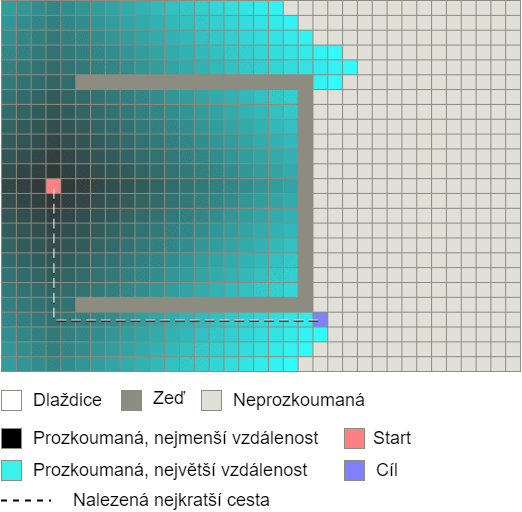
\includegraphics[width=0.47\textwidth]{Dijkstra}\label{fig:dijkstra}}
	\hfill
	\subfloat[A* algoritmus.]{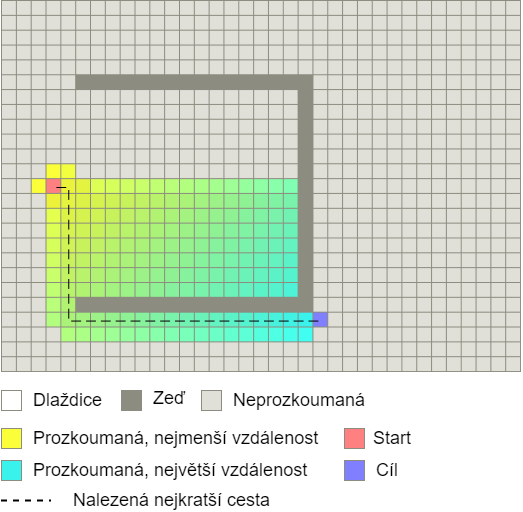
\includegraphics[width=0.47\textwidth]{AStar}\label{fig:astar}}
	\caption{Porovnání Dijkstrova algoritmu s~algoritmem A*. Ilustrace převzaty z~článku Amita Patela \citep{site:introastar}.}
	\label{fig:astardijkstra}
\end{figure}

Problémem algoritmu A* může být vlastní heuristika. Algoritmus A* požaduje, aby heuristika splňovala dvě vlastnosti, a~to přípustnost a~monotonii. Přípustnost označuje, že hodnota heuristiky pro každý vrchol je menší než minimální délka cesty do tohoto vrcholu. Monotonie poté označuje vztah \(h(x) <= d(x,y) + h(y)\), kde \(h(x)\) je hodnota heuristiky vrcholu x a \(d(x,y)\) délka hrany z~vrcholu x do vrcholu y. Splnění těchto vlastností zajišťuje, že nalezená cesta bude optimální (přípustnost) a~každý vrchol prohledáme nejvýše jednou (monotonie). 

Naše implementace algoritmu A* používá spojení statického a~dynamického generování grafu, spolu s~tvůrcem dodaným ohodnocením hran a heuristikou. Graf, reprezentující terén úrovně, je vygenerován staticky. Tedy pro každou dlaždici je vytvořen vrchol a~každý vrchol je spojen se všemi vrcholy reprezentujícími sousední dlaždice. Dále je umožněno do grafu za běhu přidávat vrcholy a~spojovat je s~již existujícími. To je použito pro umožnění pohybu po budovách, u~kterých jsou při jejich stavbě do grafu dodány vrcholy reprezentující schůdné plochy budovy a~tyto vrcholy jsou spojeny jak mezi sebou, tak s~existujícími vrcholy grafu. 

Dynamická část generování grafu se projevuje při výpočtu vah hran. Hrany nemají pevně stanovenou váhu, místo toho je pro výpočet cesty požadováno po tvůrci hry, aby každá jednotka hledající cestu poskytla tzv. kalkulátor, který dynamicky ohodnocuje hrany a~definuje jejich průchodnost. Tento přístup nám umožňuje zachovávat pouze jeden graf, který se díky využití kalkulátorů chová jako rozdílný graf pro každý kalkulátor. 
Vzhledem k~požadavkům algoritmu A* na vztah heuristiky a~ceny hran, popsaných výše, požadujeme po tvůrci hry také poskytnutí heuristiky v~rámci kalkulátoru. Zároveň tento přístup umožňuje tvůrci místo vlastní implementace algoritmu pro hledání cesty pouze změnit poskytované hodnoty hran a/nebo heuristiky, čímž může tvůrce změnit chování naší implementace algoritmu A* pro svoji potřebu.


Naše implementace A* ovšem není jediným použitelným algoritmem pro hledání cesty v~naší platformě. Pokud tvůrci nestačí úprava váhy hran a~heuristiky, umožňuje platforma implementaci vlastního algoritmu splňujícího rozhraní \texttt{IPathFindAlg}, který bude následně používán všemi součástmi platformy. Používaný algoritmus je specifikován při startu úrovně, je tedy možné, aby i~v~jednom balíčku různé úrovně používaly různé algoritmy pro hledání cesty.

\subsection{Projektily}
Simulace projektilů je častým problémem řešeným v~RTS hrách, tedy v~typu her, který naše platforma chce podporovat. Rozhodli jsme se proto implementovat tuto funkcionalitu, umožňující výpočet počátečního směru projektilu při střelbě na pohyblivý cíl, simulaci letu se stálou gravitací a~detekci zásahů. 

\subsubsection{Typy projektilů}
Existuje několik typů simulací projektilů, rozdělených podle stupně přesnosti simulace reálného světa. Těmito typy, seřazenými podle vzrůstající realističnosti simulace, jsou:
\begin{itemize}
	\item \textit{Hitscan} (bez simulace letu),
	\item s~konstantní horizontální rychlostí (proměnlivá gravitace, bez odporu vzduchu),
	\item s~konstantní dopřednou rychlostí (konstantní gravitace, bez odporu vzduchu),
	\item s~plně realistickým chováním (konstantní gravitace, simulace odporu vzduchu).
\end{itemize}

\textbf{Hitscan projektily} jsou zvláštním typem projektilů, který má nulovou dobu letu. V~okamžiku výstřelu je proveden výpočet, zda se ve směru, kterým byl výstřel mířen, vyskytuje cíl. Pokud ano, je tomuto cíli okamžitě uděleno poškození. Hitscan projektily lze dále rozdělit podle chování po zasáhnutí prvního cíle. Projektil může být zastaven prvním cílem, nebo pokračovat dále skrz první cíl a~případně zasáhnout další cíle.

\textbf{Projektily s~konstantní horizontální rychlostí} umožňují tvůrci hry z~pohledu logiky uvažovat pouze pohyb v~rovině terénu. Jak můžeme vidět na obrázku \ref{fig:horizontalproj}, výška oblouku nemá u~tohoto druhu projektilu vliv na dobu letu, která je závislá pouze na vzdálenosti zdroje a~cíle v~rovině. Tato vlastnost umožňuje zvolit výšku oblouku tak, aby graficky vypadala \uv{dobře}. Z~pohledu vyvážení síly jednotek a~budov umožňuje tento typ projektilů jednoduše spočítat dobu letu jako \( t=\text{vzdálenost}(\text{střelec}, \text{cíl}) / v \), kde \textit{v} značí určenou rychlost projektilu. Tento typ projektilů je především vhodný pro hry odehrávají se v~jedné rovině, jako například Warcraft nebo Starcraft.

\begin{figure}[h]
	\centering
	\def\svgwidth{0.7\textwidth}
	\input{img/horizontal.pdf_tex}
	\caption{Trajektorie a~čas letu projektilu s~konstantní horizontální rychlostí.}
	\label{fig:horizontalproj}
\end{figure}

\textbf{Projektily s~konstantní dopřednou rychlostí} se pohybují po balistické křivce, určené počáteční rychlostí, směrem výstřelu a~sílou gravitace. Jak můžeme vidět na obrázku \ref{fig:forwardproj}, existují vždy nejvýše dvě trajektorie, kterými lze zasáhnout při daných hodnotách výše vyjmenovaných vlastností. Díky konstantní dopředné rychlosti a~různým délkám trajektorií vždy platí vztah \(x_1 <= x_2\) Oproti předešlým typům projektilů vyžaduje tento typ složitější výpočty pro zasažení cíle, především pohybujícího se cíle. Tyto výpočty byli v~naší platformě převzaty z~článku Forresta Smitha \citep{site:projectilecalc}. Tento článek poskytuje vzorec, podle kterého lze vypočítat směr střelby projektilu, pokud známe pozice střelce a cíle, gravitaci a~počáteční rychlost projektilu. Pohyb cíle musí být konstantní rychlostí konstantním směrem. Vzhledem k~implementaci pohybu v~naší platformě, který se odehrává po spojnicích středů dlaždic, je potřeba najít spojnici, na které se bude cíl právě vyskytovat. Tento postup je iterativní, kdy procházíme cestu cíle a~v~každém bodě změny směru počítáme dobu letu projektilu. Ve chvíli, kdy najdeme dva body, kde v~prvním bude jednotka dříve než projektil, a~v~druhém později než projektil, našli jsme požadovanou spojnici. Následně využijeme převzatý vzoreček pro spočtení směru výstřelu. Tento postup by bylo možné celý provést iterativně, kde místo použití vzorečku by jsme znovu prohledávali spojnici dvou bodů a~přibližovali se k~cíli.

\begin{figure}[h]
	\centering
	\def\svgwidth{0.7\textwidth}
	\input{img/forward.pdf_tex}
	\caption{Trajektorie a~čas letu projektilu s~konstantní dopřednou rychlostí.}
	\label{fig:forwardproj}
\end{figure}

\textbf{Projektily s~realistickým chováním} přidávají oproti předchozímu typu ještě jednu vlastnost, a~to odpor vzduchu. Jak můžeme při porovnání trajektorií na obrázcích \ref{fig:forwardproj} a \ref{fig:withdragproj}, má trajektorie tohoto typu projektilu složitější tvar.  Výpočet tohoto typu projektilů je nejčastěji prováděn iterativně, kdy je odhadnuta doba letu, podle této doby letu je predikován pohyb cíle, a~následně spočítána opravdová délka letu. Tento postup je opakován do dosažení potřebné přesnosti.

\begin{figure}[h]
	\centering
	\def\svgwidth{0.7\textwidth}
	\input{img/withdrag.pdf_tex}
	\caption{Trajektorie a~čas letu projektilu s~plně realistickým chováním.}
	\label{fig:withdragproj}
\end{figure}


Podle priorit a~zasazení hry jsou často voleny méně realistické modely, které z~pohledu hry mohou mít výhody oproti plně realistickému chování. Těmito výhodami může být lepší zasazení do tématu hry, což můžeme vidět u~laserových zbraní v~sci-fi hrách jako Starcraft~2 \citep{site:starcraft}, které jsou typu \textit{Hitscan}. I~když by se zdálo, že je vždy nejlepší co nejvíce se blížit realitě a~tedy vybrat si plně realistické chování, v~některých hrách je důležitější možnost vyvážení síly jednotek, předvídatelnosti chování a/nebo vzhledu.  


Naše platforma poskytuje implementaci výpočtu směru střelby pro projektily s~konstantní dopřednou rychlostí a~simulaci letu tohoto typu projektilů. Naším cílem ovšem bylo nijak neomezovat tvůrce her, kvůli čemuž jsou tyto prvky poskytovány jako komponenty, které lze připojit k~projektilu a~které následně řídí jeho chování. Nijak ale nejsou provázány s~vlastní třídou projektilu, čímž je tvůrcům hry umožněno implementovat kterýkoli z~typů projektilů.


